\section{Include dan Require: Mengorganisasi Kode dalam Banyak File}

Seiring bertambahnya kompleksitas proyek web, menulis seluruh kode dalam satu file menjadi tidak praktis dan sulit dipelihara. PHP menyediakan empat pernyataan untuk menyisipkan kode dari file lain: \code{include}, \code{require}, \code{include\_once}, dan \code{require\_once}. Keempat pernyataan ini memungkinkan Anda memecah kode menjadi file-file terpisah sesuai fungsinya --- misalnya file konfigurasi, file fungsi utilitas, file header, dan file footer --- sehingga kode lebih terorganisir dan mudah digunakan ulang \cite{phpManual}.

Perbedaan utama antara \code{include} dan \code{require} terletak pada penanganan error ketika file yang disisipkan tidak ditemukan. \code{include} hanya menghasilkan \textit{warning} (E\_WARNING) dan eksekusi skrip tetap berlanjut; \code{require} menghasilkan \textit{fatal error} (E\_COMPILE\_ERROR) dan menghentikan eksekusi. Versi \code{\_once} memastikan file hanya disisipkan satu kali meskipun pernyataan dipanggil berkali-kali, mencegah duplikasi definisi fungsi atau kelas yang menyebabkan error \cite{phpRightWay}.

\begin{table}[ht]
\centering
\begin{tabular}{|P{3cm}|P{3.5cm}|P{3cm}|P{2.5cm}|}
\hline
\textbf{Pernyataan} & \textbf{Jika File Tidak Ada} & \textbf{Duplikasi} & \textbf{Penggunaan} \\
\hline
\code{include} & Warning, lanjut & Boleh berulang & Template HTML \\
\hline
\code{require} & Fatal error, berhenti & Boleh berulang & File kritis \\
\hline
\code{include\_once} & Warning, lanjut & Sekali saja & Library opsional \\
\hline
\code{require\_once} & Fatal error, berhenti & Sekali saja & Konfigurasi, class \\
\hline
\end{tabular}
\caption{Perbandingan include, require, dan variannya}
\end{table}

Dalam praktik, \code{require\_once} paling sering digunakan untuk menyisipkan file konfigurasi, definisi fungsi, dan definisi kelas, karena file-file ini kritis (harus ada) dan tidak boleh diduplikasi. \code{include} biasanya digunakan untuk menyisipkan template HTML (header, footer, sidebar) yang bersifat opsional. Berikut contoh pengorganisasian kode proyek web sederhana.

\begin{webcode}[language=PHP, caption={Struktur proyek dengan include dan require}]
<?php
// File: config.php (konfigurasi database)
$db_host = "localhost";
$db_name = "toko_online";
$db_user = "root";
$db_pass = "";
?>
\end{webcode}

\begin{webcode}[language=PHP, caption={File utama menggunakan require dan include}]
<?php
// File: index.php (halaman utama)

// File kritis: gunakan require_once
require_once 'config.php';
require_once 'functions.php';

// Template: gunakan include
include 'templates/header.php';
?>

<main>
  <h1>Selamat Datang di <?= htmlspecialchars($site_name) ?></h1>
  <p>Konten halaman utama...</p>
</main>

<?php include 'templates/footer.php'; ?>
\end{webcode}

Mengorganisasi kode ke dalam file terpisah memiliki banyak keuntungan: kode lebih mudah dibaca, perubahan pada satu komponen tidak memengaruhi file lain, dan komponen yang sama (seperti header/footer) dapat digunakan ulang di banyak halaman tanpa duplikasi. Berikut diagram struktur folder proyek web PHP yang terorganisir dengan baik.

\begin{figure}[ht]
\centering
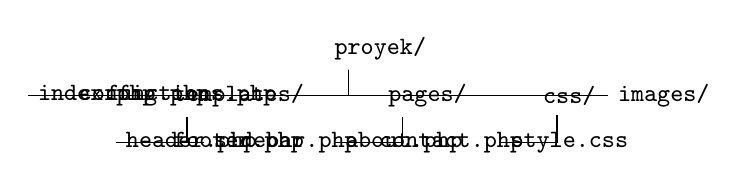
\begin{tikzpicture}[
  every node/.style={font=\small\ttfamily},
  level distance=0.6cm,
  sibling distance=0.6cm,
  edge from parent path={(\tikzparentnode.south west) ++ (0.3,0) |- (\tikzchildnode.west)},
  level 1/.style={level distance=0.6cm, sibling distance=0.6cm},
  level 2/.style={level distance=0.6cm, sibling distance=0.6cm}
]
  \node {proyek/}
    child {node {index.php}}
    child {node {config.php}}
    child {node {functions.php}}
    child {node {templates/}
      child {node {header.php}}
      child {node {footer.php}}
      child {node {sidebar.php}}
    }
    child [missing] {}
    child [missing] {}
    child [missing] {}
    child {node {pages/}
      child {node {about.php}}
      child {node {contact.php}}
    }
    child [missing] {}
    child [missing] {}
    child {node {css/}
      child {node {style.css}}
    }
    child [missing] {}
    child {node {images/}};
\end{tikzpicture}
\caption{Contoh struktur folder proyek web PHP}
\end{figure}

\begin{konsep}
\textbf{Prinsip DRY (Don't Repeat Yourself):} Jika Anda menyalin-tempel kode yang sama ke banyak file, itu adalah tanda bahwa kode tersebut harus diekstrak ke file terpisah dan disisipkan dengan \code{include}/\code{require}. Prinsip DRY memastikan setiap potongan logika hanya ada di satu tempat, sehingga perbaikan bug atau perubahan fitur cukup dilakukan sekali \cite{phpRightWay}.
\end{konsep}

